\section{Thực hiện phần cứng (Hardware Implementation)}
\label{sec:hardware_implementation}

Việc triển khai phần cứng của hệ thống Phát hiện té ngã và Cảnh báo (FDAS) được thực hiện dựa trên kiến trúc mô-đun, với hai module chính hoạt động độc lập nhằm đảm bảo tính linh hoạt và khả năng bao phủ giám sát rộng. Cấu trúc mô-đun này cho phép hệ thống duy trì hoạt động ngay cả khi một module gặp sự cố, đồng thời tăng cường độ chính xác bằng cách phối hợp dữ liệu từ cảm biến chuyển động và hình ảnh để giảm thiểu các cảnh báo sai. Module thứ nhất tập trung vào việc thu thập dữ liệu chuyển động và định vị, trong khi module thứ hai được thiết kế để xử lý và phân tích hình ảnh.

\subsection{Module I: Thiết bị đeo\slash Cảm biến}
\label{ssec:module_one}

Module này đóng vai trò là thiết bị phát hiện ban đầu, được thiết kế nhỏ gọn để người dùng có thể mang theo. Nó bao gồm các thành phần cốt lõi sau:

\begin{figure}[H]
 	\centering
 	\includegraphics[width=0.7\textwidth]{figures/module1_block_diagram-crop.pdf}
 	\caption{Sơ đồ khối Module I: Thiết bị đeo\slash Cảm biến}
 	\label{fig:module1_block_diagram}
\end{figure}

\begin{itemize}
 	\item \textbf{Bộ vi điều khiển ESP32-DevKitC-1}: Được chọn làm trung tâm xử lý chính nhờ vào hiệu suất ổn định và các giao thức kết nối không dây (Wi-Fi, Bluetooth) tích hợp. So với các vi điều khiển phổ biến khác như STM32, ESP32 có lợi thế về chi phí và khả năng kết nối mạng, giúp việc truyền dữ liệu lên máy chủ trở nên dễ dàng hơn.
 	\item \textbf{Cảm biến MPU6050}: Đây là một \textbf{bộ đo lường quán tính (IMU) 6 trục} bao gồm cảm biến gia tốc và con quay hồi chuyển. MPU6050 được sử dụng rộng rãi trong các dự án IoT nhờ độ chính xác cao và tích hợp bộ xử lý chuyển động kỹ thuật số (DMP), giúp giảm tải cho vi điều khiển chính. MPU6050 đo lường các thay đổi về gia tốc và tốc độ góc, cho phép phát hiện chính xác các chuyển động bất thường, đặc trưng của một cú ngã.
 	\item \textbf{Module GPS và 4G (EC800K)}: Module tích hợp này cung cấp khả năng định vị và kết nối di động. \textbf{GPS} thu thập tọa độ địa lý, cho phép xác định vị trí người dùng khi sự kiện xảy ra ngoài trời hoặc các khu vực không được bao phủ bởi camera. \textbf{Module 4G} đảm bảo tín hiệu cảnh báo được gửi đến máy chủ xử lý mà không cần phụ thuộc vào mạng Wi-Fi, tăng cường tính di động của hệ thống, đặc biệt hữu ích khi người dùng ở xa nhà.
 	\item \textbf{Các thành phần bổ trợ}: Một \textbf{còi báo (buzzer)} và một \textbf{đèn LED onboard} được sử dụng để cung cấp phản hồi ngay lập tức cho người dùng, thông báo về trạng thái của thiết bị hoặc khi một sự kiện té ngã được phát hiện.
\end{itemize}

\begin{figure}[H]
 	\centering
 	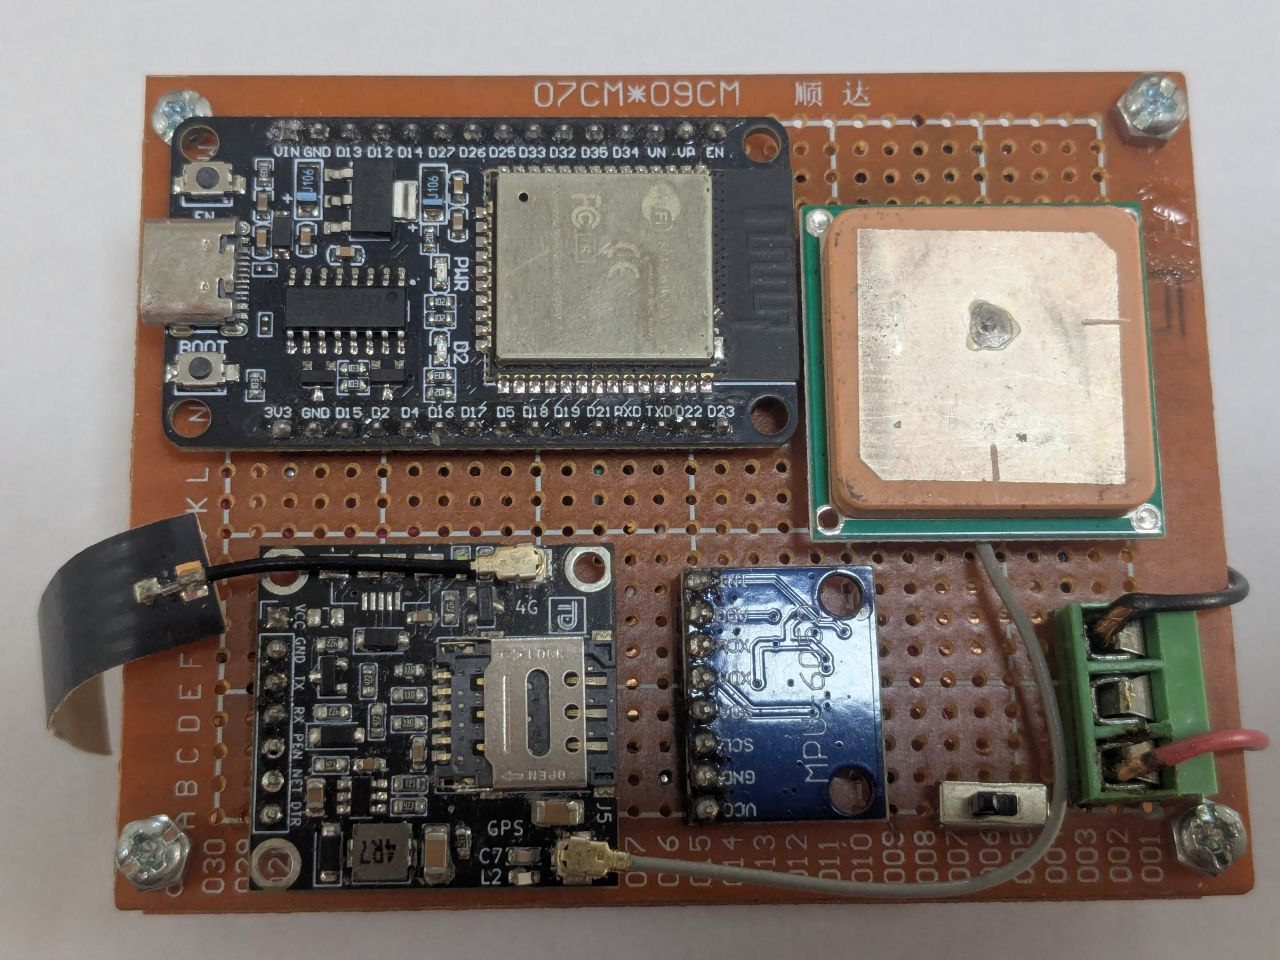
\includegraphics[width=0.8\textwidth]{figures/real_board1.jpg}
 	\caption{Hình ảnh thực tế Module I đã hoàn thiện}
 	\label{fig:module1_photo}
\end{figure}

Sơ đồ nguyên lý chi tiết (schematic) của Module I được vẽ bằng phần mềm KiCad và được đính kèm trong \textbf{Phụ lục B}.

\subsection{Module II: Camera giám sát}
\label{ssec:module_two}

Module này đóng vai trò xác nhận sự kiện té ngã bằng hình ảnh. Nó được đặt ở các khu vực giám sát trọng yếu như phòng khách sảnh hoặc phòng sinh hoạt chung. Các thành phần chính bao gồm:

\begin{figure}[H]
 	\centering
 	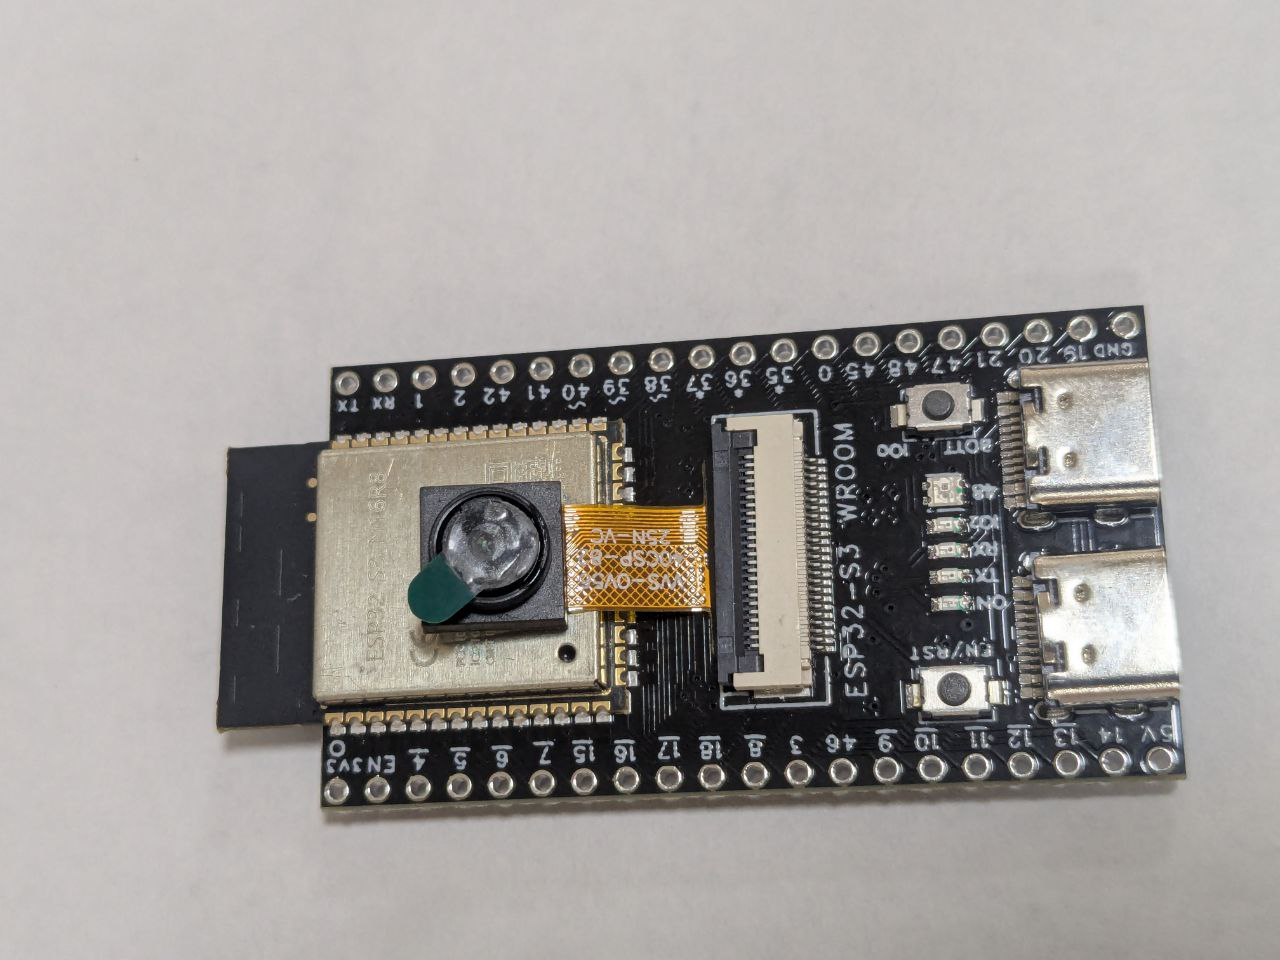
\includegraphics[width=0.8\textwidth]{figures/real_board2.jpg}
 	\caption{Hình ảnh thực tế Module II}
 	\label{fig:module2_photo}
\end{figure}

\begin{itemize}
 	\item \textbf{Bộ vi điều khiển ESP32-S3-N16R8}: Được lựa chọn do có bộ xử lý mạnh mẽ hơn và dung lượng bộ nhớ lớn hơn (16MB Flash và 8MB PSRAM), cần thiết để xử lý luồng dữ liệu hình ảnh nặng từ camera. ESP32-S3 là lựa chọn tối ưu về chi phí cho các ứng dụng xử lý hình ảnh IoT so với các vi điều khiển khác có cùng khả năng.
 	\item \textbf{Module camera OV5640}: Đây là một cảm biến camera 5MP có khả năng chụp ảnh và quay video chất lượng cao. Việc lựa chọn OV5640 thay vì các camera có độ phân giải thấp hơn như OV2640 là để đảm bảo chất lượng hình ảnh đủ tốt cho việc phân tích bằng các thuật toán Python trên máy chủ, giúp xác nhận sự kiện té ngã và giảm thiểu các cảnh báo sai một cách hiệu quả.
\end{itemize}

\subsection{Bảng tổng hợp các thành phần phần cứng}
\label{ssec:component_summary}

Bảng \ref{tab:hardware_components} dưới đây tóm tắt các thành phần chính của hai module, cùng với vai trò và giá thành ước tính của chúng trong hệ thống.

\begin{table}[H]
 	\centering
 	\caption{Tổng hợp các thành phần phần cứng}
 	\label{tab:hardware_components}
 	\begin{tabular}{|l|p{5cm}|p{2cm}|l|}
 	 	\hline
 	 	\textbf{Thành phần} & \textbf{Chức năng} & \textbf{Hình ảnh} & \textbf{Giá thành ước tính (VNĐ)} \\
 	 	\hline
 	 	ESP32-DevKitC-1 & Bộ vi điều khiển chính & 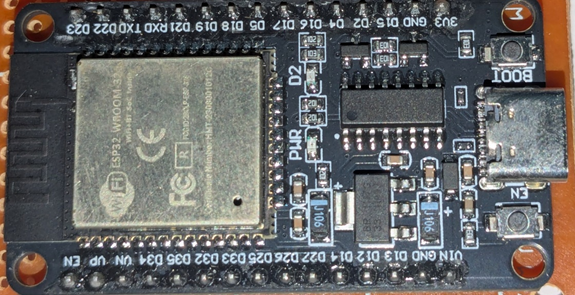
\includegraphics[width=2cm]{figures/real_esp32_c1.png} & 110.000 - 125.000 \\
 	 	\hline
 	 	MPU6050 & Cảm biến IMU 6 trục & 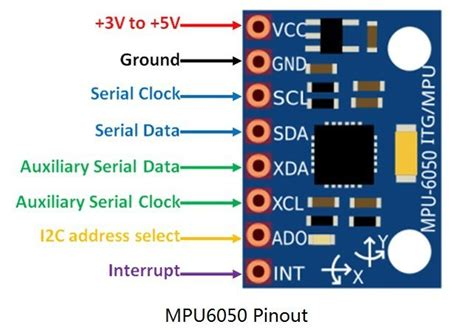
\includegraphics[width=2cm]{figures/real_mpu6050.jpg} & 45.000 - 55.000 \\
 	 	\hline
 	 	GPS-antenna & Anten nhận tín hiệu GPS & 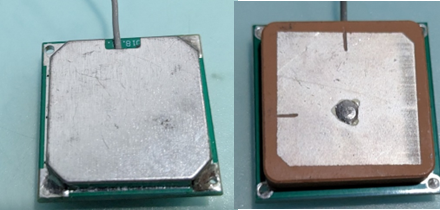
\includegraphics[width=2cm]{figures/real_gps_antenna.png} & 35.000 - 60.000 \\
 	 	\hline
 	 	Module GPS/4G (EC800K) & Định vị và gửi tín hiệu cảnh báo & 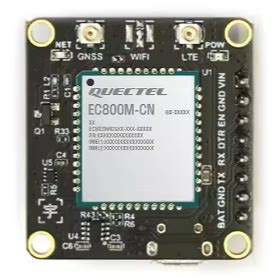
\includegraphics[width=2cm]{figures/real_ec800k.jpg} & ~240.000 \\
 	 	\hline
 	 	Buzzer & Cảnh báo âm thanh & 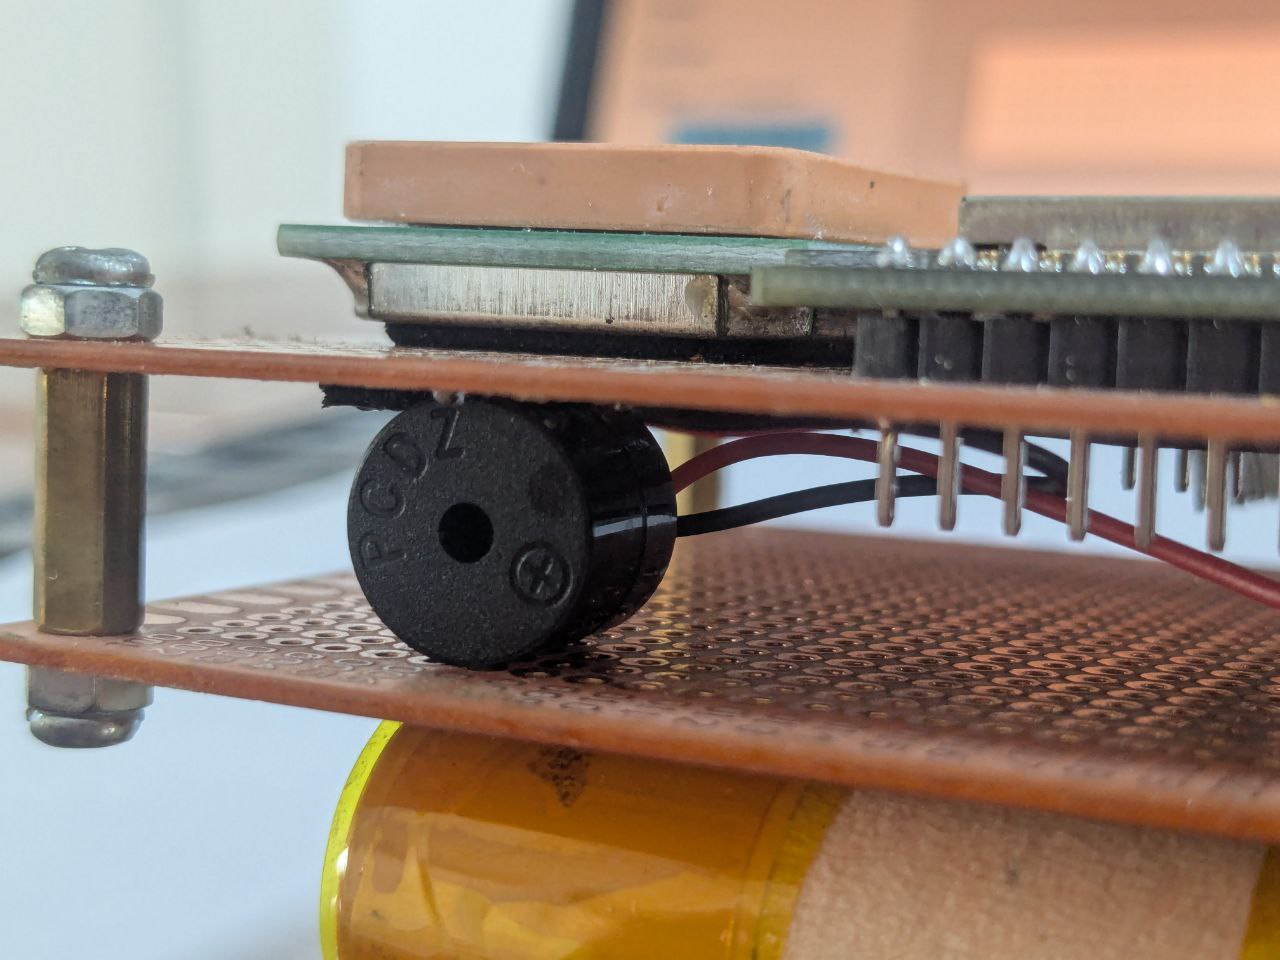
\includegraphics[width=2cm]{figures/real_buzzer.jpg} & 5.000 - 10.000 \\
 	 	\hline
 	 	ESP32-S3-N16R8 & Bộ vi điều khiển cho xử lý hình ảnh & 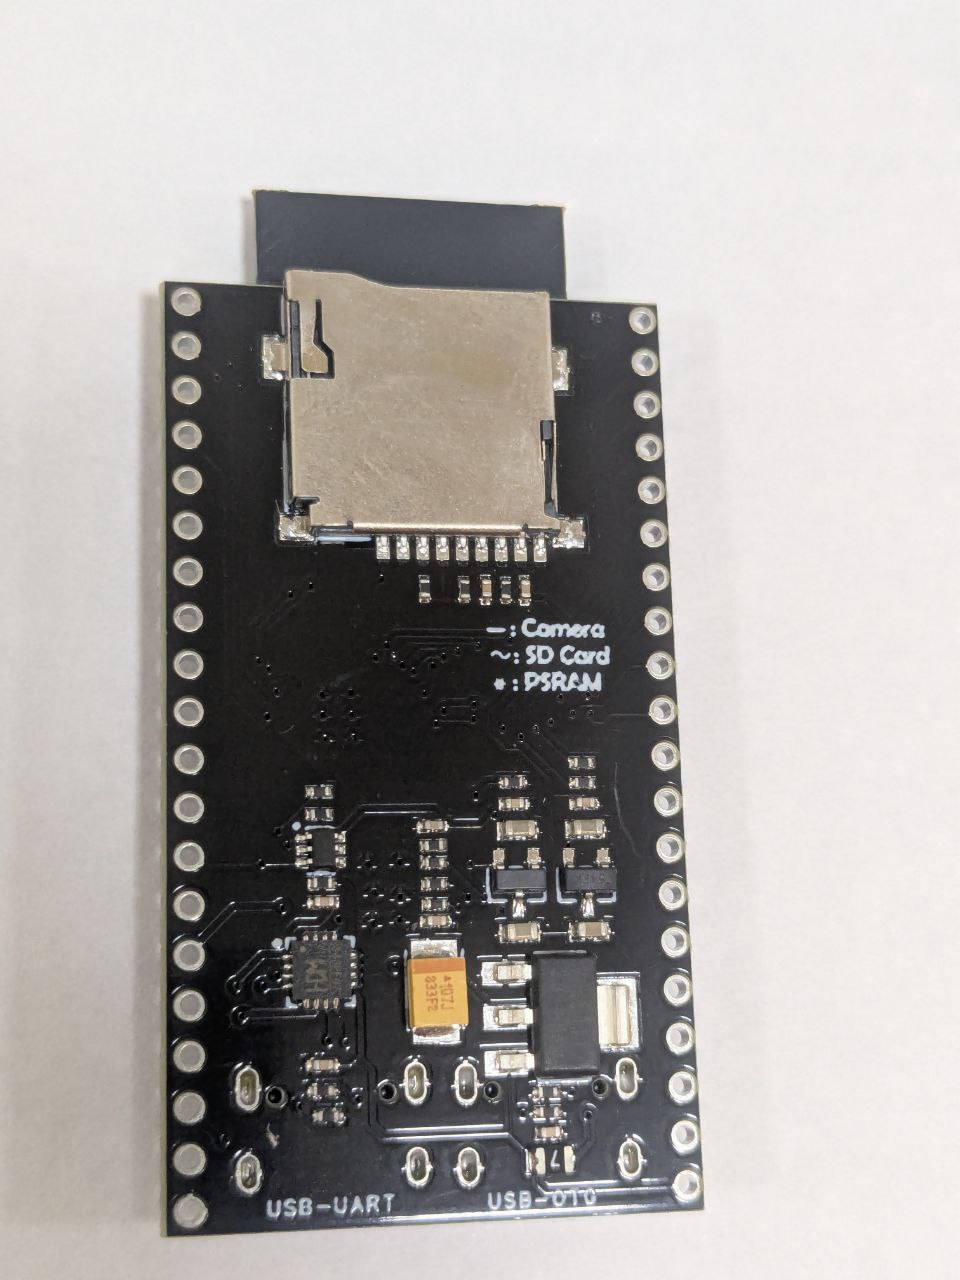
\includegraphics[width=2cm]{figures/real_esp32_s3_2.jpg} & 275.000 - 300.000 \\
 	 	\hline
 	 	Camera OV5640 & Cảm biến hình ảnh 5MP & 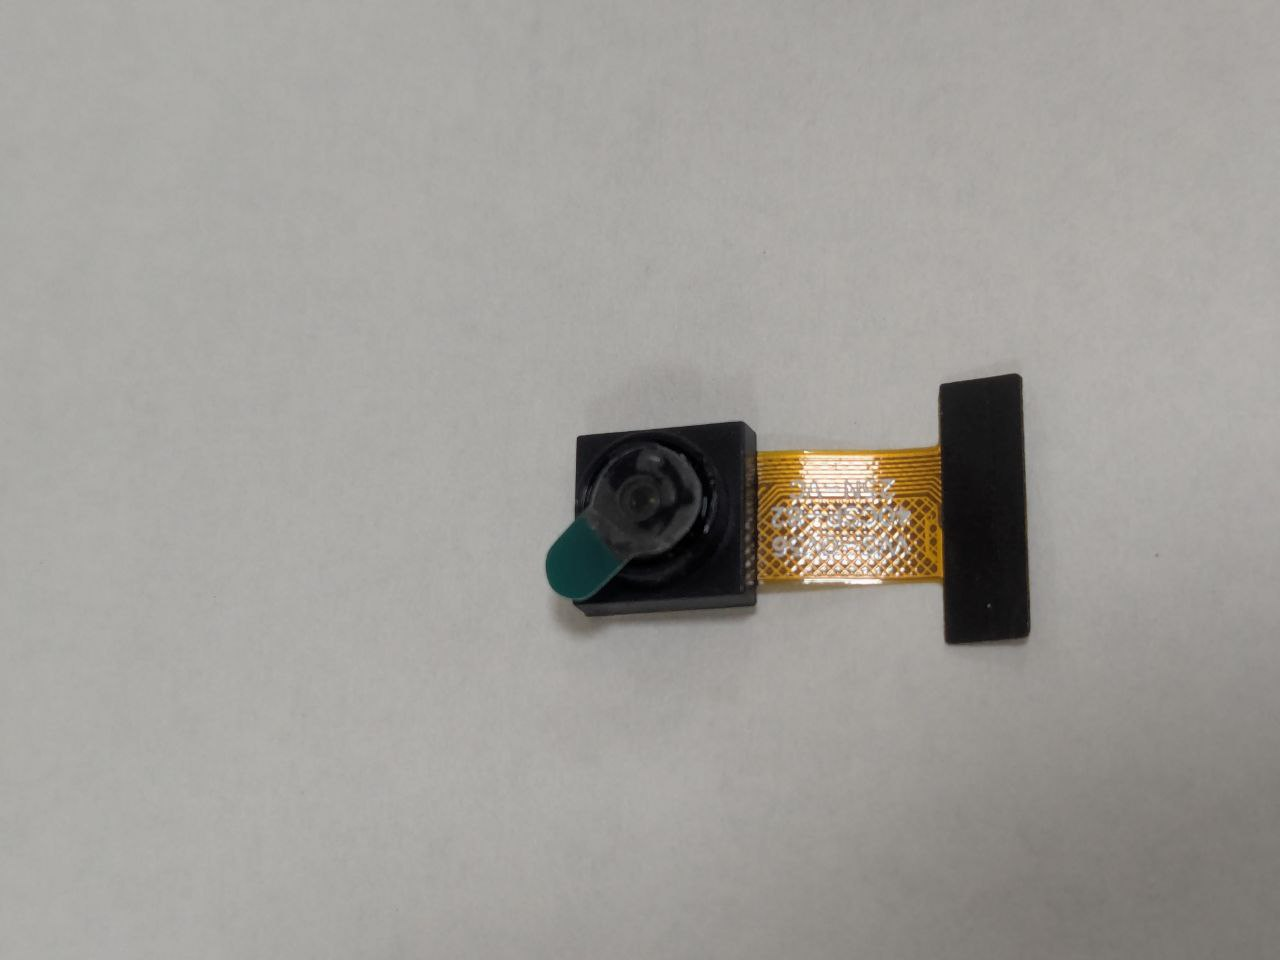
\includegraphics[width=2cm]{figures/real_ov5640.jpg} & 150.000 - 200.000 \\
 	 	\hline
 	\end{tabular}
\end{table}

